%----------------------------------------------------------------------------------------
%	SECTION 1.1
%----------------------------------------------------------------------------------------

\section{The Quotient Topology}

\begin{definition}
    Let $X$ and  $Y$ be topological spaces, and let  $p:X \rightarrow Y$ be onto. We say that  $p$
    is a \textbf {quotient map} if a subset $U \subseteq Y$ is open if and only if  $p^{-1}(U)
    \subseteq X$ is open. We say that a subset $C$ is \textbf {saturated} with respect to $p$
    if for every $p^{-1}(\{y\})$ that intersects $C$,  $p^{-1}(\{y\}) \subseteq C$; that is $C \cap
    p^{-1}(\{y\})=p^{-1}(\{y\})$.
\end{definition}

\begin{figure}[h]
    \centering
    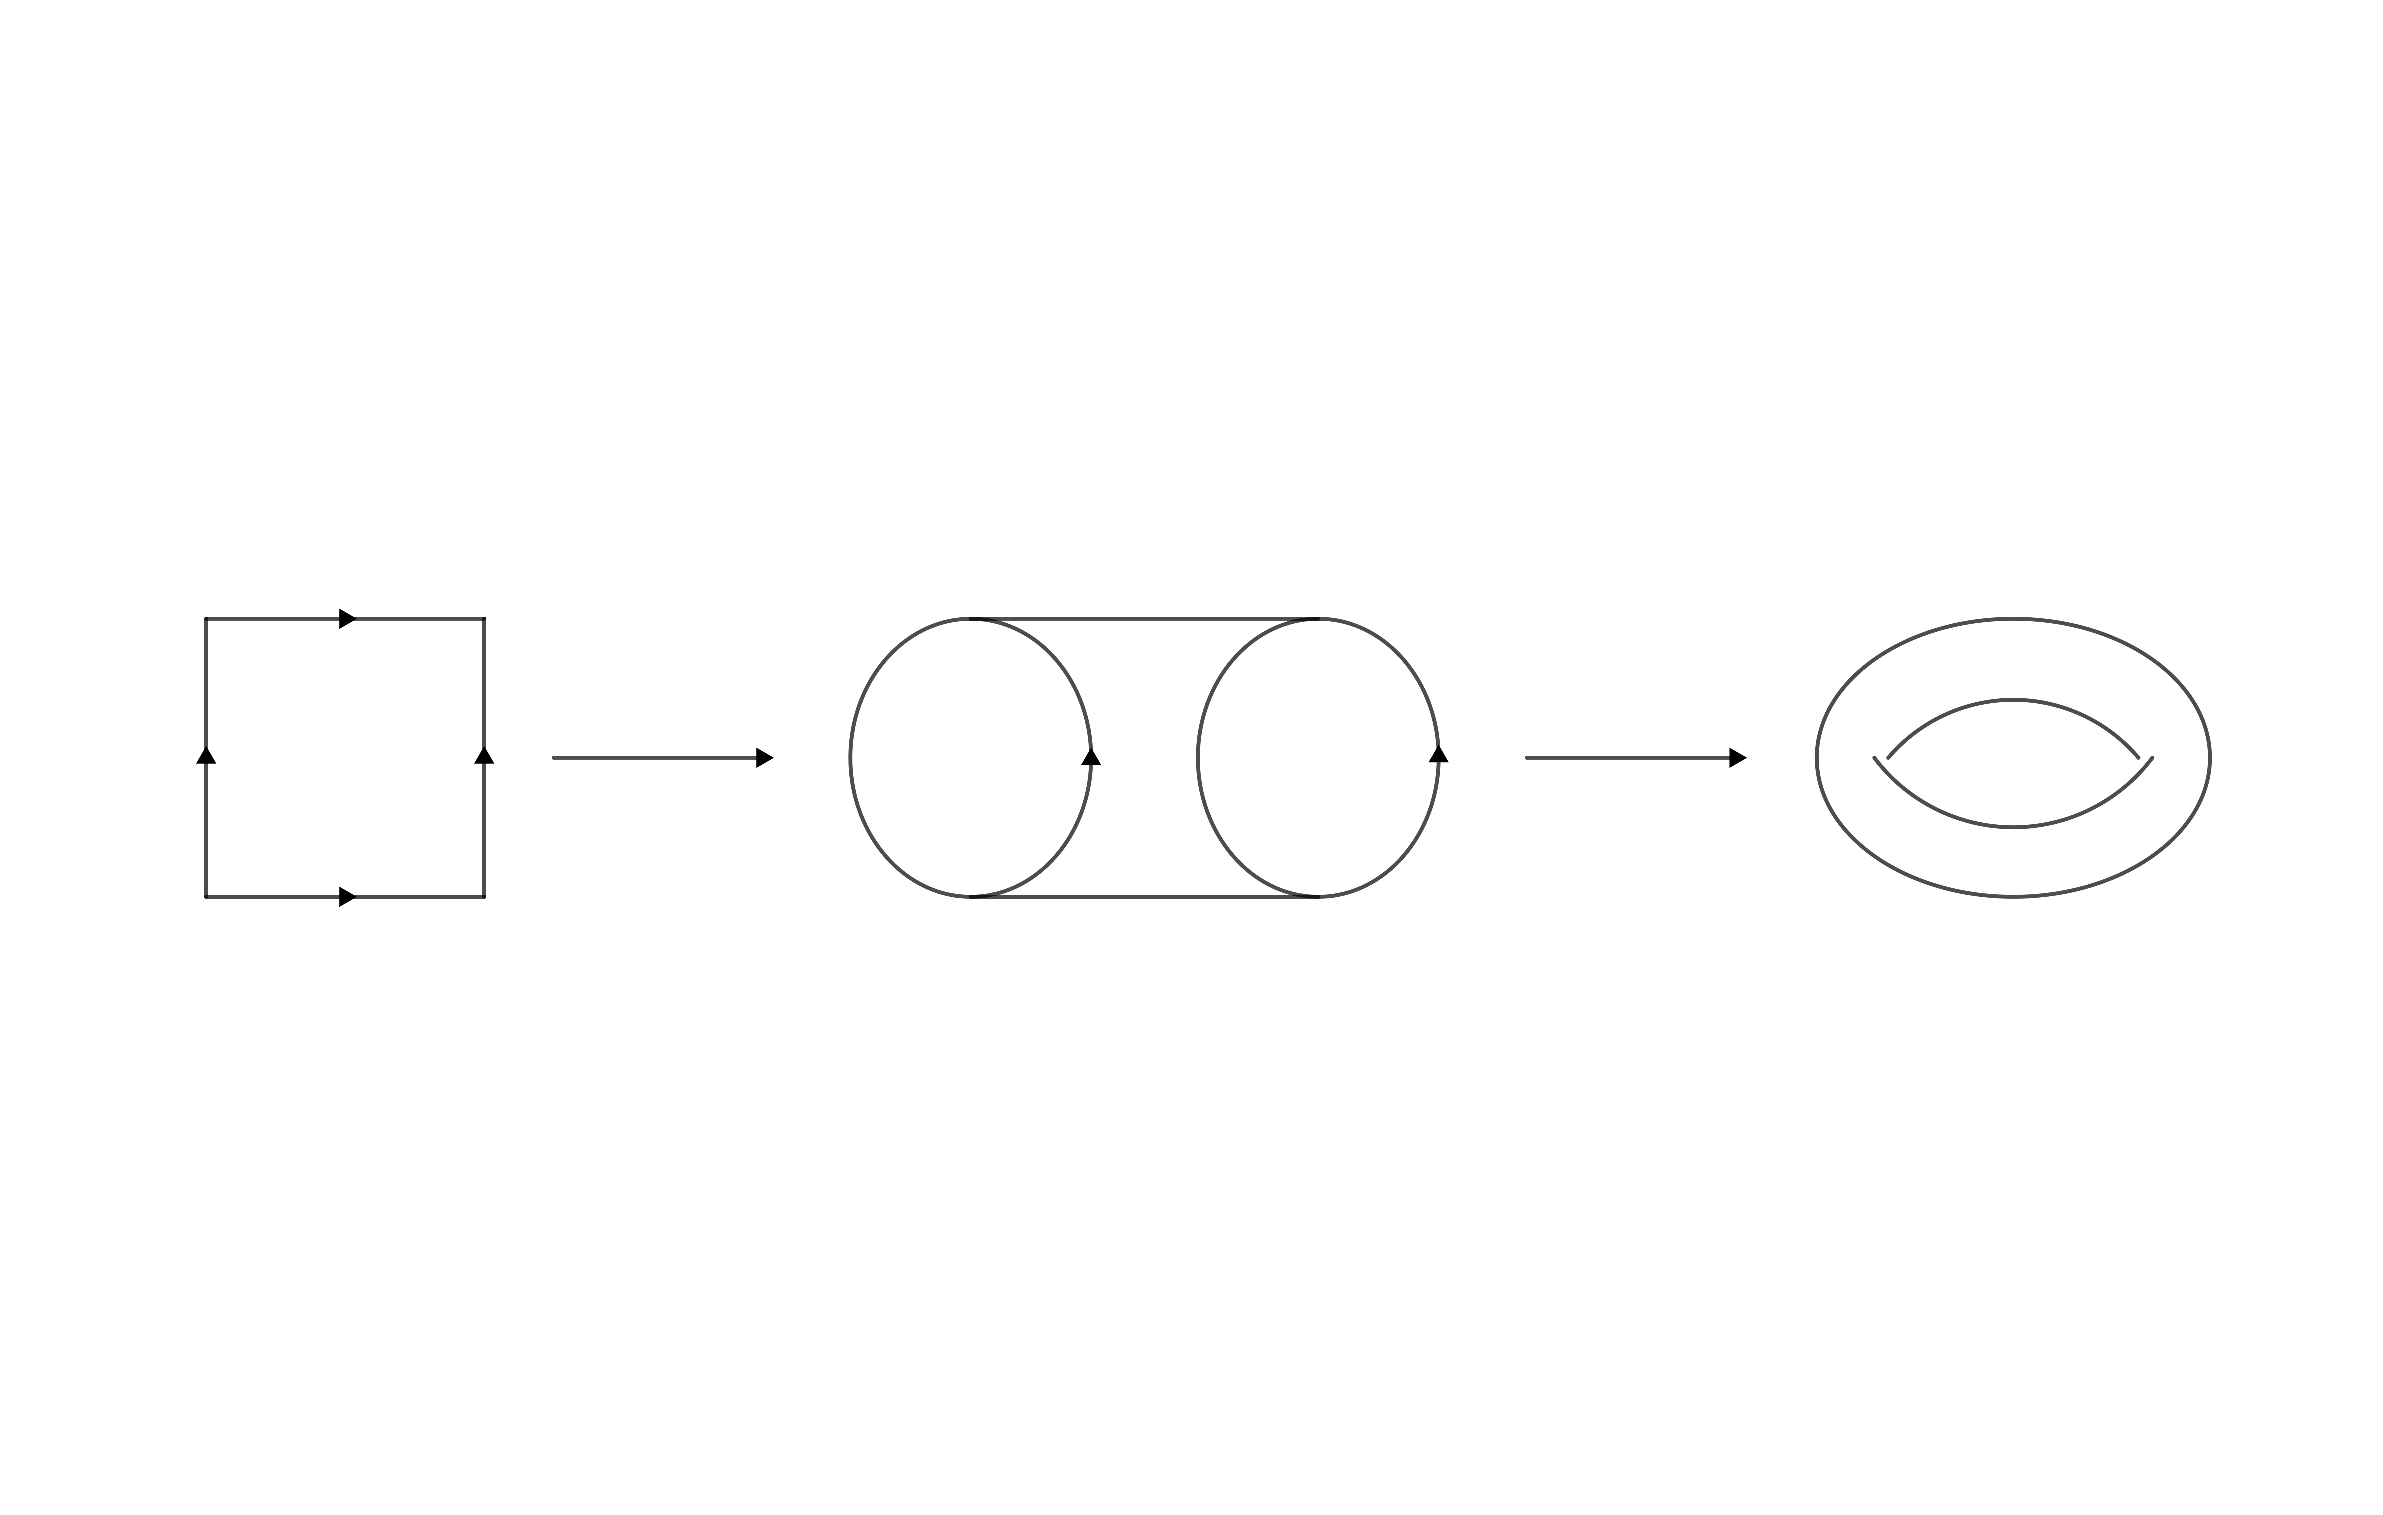
\includegraphics[scale = 0.3]{Figures/Chapter2/squareToCylinderToTorus.eps}
    \caption{Gluing the edges of the unit square to form a cylinder, and then a torus.}
    \label{fig_2.2}
\end{figure}

\begin{definition}
    Let $f:X \rightarrow Y$ be a map, with $X$ and  $Y$ topological spaces. We say that  $f$ is an
    \textbf {open map} if for each open subset $U \subseteq X$,  $f(U) \subseteq Y$ is also open. We say $f$ is a
    \textbf {closed map} if for each closed subset $U \subseteq X$,  $f(U) \subseteq Y$ is closed.
\end{definition}

\begin{lemma}\label{4.4.1}
    If $p:X \rightarrow Y$ is a continuous map of  $X$ onto  $Y$, for topological spaces  $X$ and
    $Y$, that is either open or closed, then  $p$ is a quotient map.
\end{lemma}
\begin{remark} 
    A quotient map need not be open nor closed.		
\end{remark}

\begin{example}
    \begin{enumerate}[label=(\arabic*)]
        \item Let $X$ be the subspace  $[0,1] \cup [2,3]$ and $Y$ be the subspace  $[0,2]$ in $\R$,
            and defined  $p:X \rightarrow Y$ by  $p(x)=\begin{cases}
                                                x, \text{ } x \in [0,1] \\
                                                x-1, \text{ } x \in [2,3] \\
                                            \end{cases}$.
        We have that $p$ is continuous onto, by the pasting lemma, furthermore,  $p$ is also closed;
        hence  $p$ is a quotient map.  $p$ is not open however, as  $p([0,1])=[0,1]$ is closed in
        $Y$.

        Now if  $A$ is the subspace  $[0,1) \cup [2,3]$ of $X$, then  $\:A \rightarrow Y$ is
        continuous onto, but fails to be closed. So  $p|_A$ is not a quotient map, depsite the fact
        that  $[2,3]$ is open in $A$ and saturated with respect to  $p|_A$.

        \item Let $\pi_1:\R \times \R \rightarrow \R$ be the projection map that takes $x \times y
            \rightarrow x$. Clearly  $\pi_1$ is continuous onto, and $\pi_1$ is also open as
            $\pi_1(U \times V)=U$ which is open in $Y$; hence  $\pi_1$ is a quotient map. Now
            consider the closed set $C=\{x \times y:xy=1\}$ in $\R \times \R$.
            $\pi_1(C)=\com{\R}{\{0\}}$ which is not closed.
    \end{enumerate}
\end{example} 

\begin{theorem}\label{2.4.2}
    Let $X$ be a topological space, and  $A$ a set, and let  $p:X \rightarrow Y$ be onto. Define
    $\Tc$ to be the collection of subsets  $U$ of  $A$ for which  $p^{-1}(U)$ is open in $X$. Then
    $\Tc$ is a unique topology for which  $p$ is a  quotient map.
\end{theorem}
\begin{proof}
    Clearly $\emptyset,A \in \Tc$, for  $p^{-1}(\emptyset)=\emptyset$ and $p^{-1}(A)=X$. Now let
    $\{U_{\alpha}\}$ and $\{U_i\}_{i=1}^{n}$ be collections of subsets of $A$. Then
        \begin{equation*}
            p^{-1}(\bigcup{U_{\alpha}})=\bigcup{p^{-1}(U_{\alpha})}
        \end{equation*}
    and 
        \begin{equation*}
            p^{-1}(\bigcap_{i=1}^{n}{U_i})=\bigcap_{i=1}^{n}{p^{-1}(U_i)}.
        \end{equation*}
    Thus $\Tc$ is a topology on  $A$. Now notice that this also makes  $p$ into a quotient map.

    Now suppose that there is another topology $\Tc'$ for which  $p$ is a quotient map.  Clearly $\Tc
    \subsesubseteq \Tc'$, now if $p$ is open, then for $U$ open in $X$,  $p(U)$ is open in $A$,
    hence so are their preimages, and since $p$ is continuous and onto this makes $\Tc' \subseteq
    \Tc$, thus $\Tc$ is unique. Likewise, by similar reasoning with closed sets, if  $p$ is closed,
     $\Tc$ is still unique.
\end{proof}

\begin{definition}
    If $X$ is a topologicas space, and  $A$ a set, and  $p:X \rightarrow A$ is onto, then there is
    exactly one topology  $\Tc$ on  $A$ for which  $p$ is a quotient map. We call this topology the
    \textbf {quotient topology} on $A$ induced by  $p$.
\end{definition}

\begin{example}
    Let $p:\R \rightarrow A$, with  $A=\{a,b,c\}$ be defined by
        \begin{equation*}
            p(x)=\begin{cases}
                    a, \text{ } x>0 \\
                    b, \text{ } x<0 \\
                    c, \text{ } x=0 \\
                \end{cases}
        \end{equation*}
    Then the quotient topology on $A$ is the topology  $\Tc=\{\emptyset, \{a\}, \{b\}, \{a,b\},A\}$.
    
    \begin{figure}[h] 
        \centering
        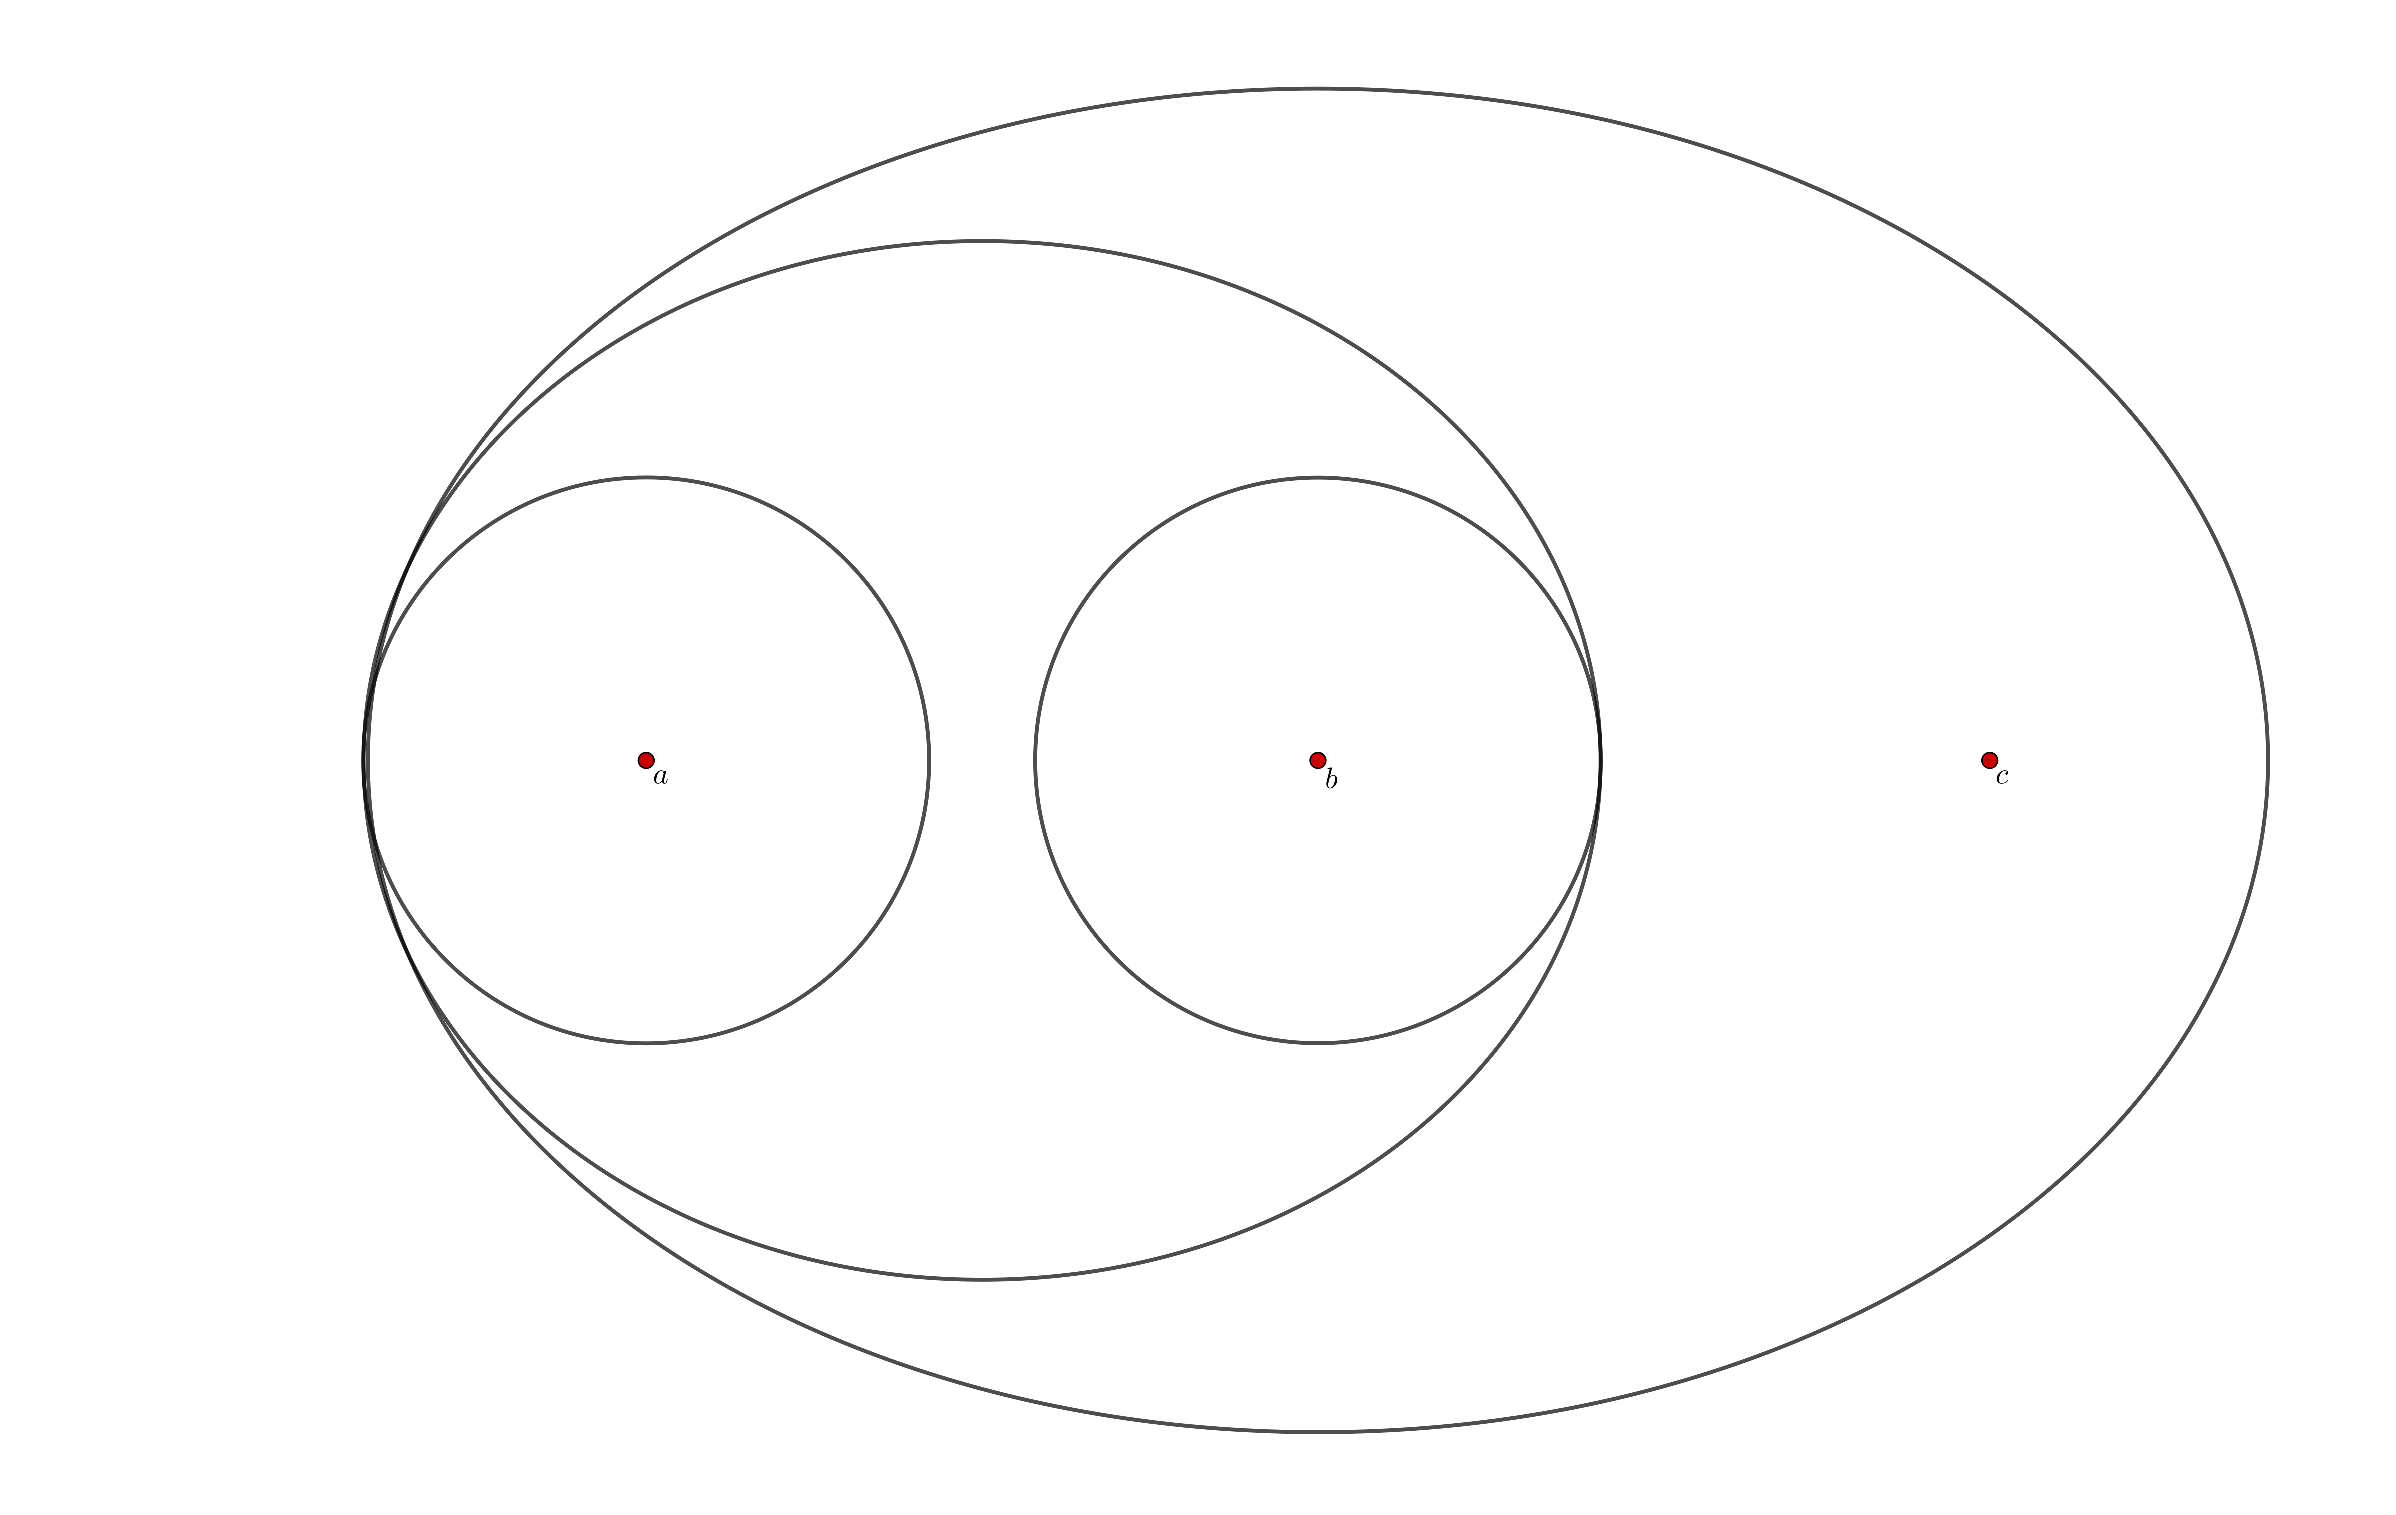
\includegraphics[scale = 0.2]{Figures/Chapter2/quotientOnABC.eps}
        \caption{The quotient topology on $A=\{a,b,c\}$ induced by $p$.}
    \end{figure}
\end{example} 

\begin{definition}
    Let $X$ be a topological space and  $X/p$ be a partition of  $X$ into disjoint subsets whos
    disjoint union is  $X$. Let  $p:X \rightarrow X/p$ be onto such that  $p:x \rightarrow U$ if  $x
    \in U$. We call  $X/p$ in the quotient topology induced by $p$ the \textbf{quotient space} of $X$, or the 
    \textbf{decomposition space} of $x$.
\end{definition}

We can take an equivalence relation $\sim$ on  $X$ by taking  $x \sim y$ if  $x,y \in U$ for  $U \in
X/p$. Then the quotient space is the collection of equivalence classes of $X$; that is we can think
of obtaining $X^*$ by ``identify'' those pairs of equivalent points. Similarly, we can also describe
the quotient space $X/p$ by noting a subset $U$ of equivalence classes where $p^{-1}(U)=\bigcup_{V
\in U}{V}$ is the union of all equivalence classes in $U$. We will denote the quotient space by
$X/p$ or  $X/\sim$.

\begin{example}
    \begin{enumerate}[label=(\arabic*)]
        \item     Let $X=\{x \times y: x^+y^2 \leq 1\}$ be the closed unit ball in $\R^2$ and let  $X/\sim$ be the
    quotient space of  $X$ by taking its equivalence classes to be all one point sets  $\{x \times
    y\}$ for which $x^2+y^2<1$, and the unit circle  $S^1$. Take  $p:X \rightarrow X/\sim$ by the
    rule
        \begin{equation*}
            p:x \times y \rightarrow \begin{cases}
                \{x \times y\}, & x^2+y^22<1 \\
                S^1        & x^2+y^2=1 \\ 
                      \end{cases}
        \end{equation*}
    Clearly $p$ is onto by definition, and e have that for any one point sets and  $ S_1$ in
    $X/\sim$ that  $p^{-1}(\{x \times y\})=B_{||\cdot||}(x,1)$, and $p^{-1}(S^1)=S_1$, thus open
    sets in $X$ are open in  $X/\sim$  (likewise closed), so $p$ is open which makes it into a
    quotient map. Now let  $S^2=\{x \times y \times z: x^2+y^2+z^2=1\}$ be the \textbf{unit sphere}
    in $\R^3$, then we can map  $X/\sim \rightarrow S^2$ by taking  $\{x \times y\} \rightarrow \{x
    \times y \times z: x^2+y^2+z^2<1\}$ and $ S^1 \rightarrow S^1$. Then we have that $X/\sim$ is
    homeomorphic to the unit sphere.		
    \end{enumerate}

        \item Let $X$ be the unit square  $[0,1] \times [0,1]$ and define the quotient space
            $X/\sim$ of $X$ to be the collection of all point sets $\{x \times y\}$ for which $x
            \times y \in (0,1) \times (0,1)$, together with the sets $\{x \times 0, x \times 1\},
            \{0 \times y, 1 \times y\}$ with $x \times y \in (0,1) \times (0,1)$, and the set $\{0
            \times 0, 0 \times 1, 1 \times 0, 1 \times 1\}$, then we can show that $X/\sim$ is
            homeomorphic to a torus.
\end{example} 

\begin{figure}[h] 
    \centering
    \includegraphics[scale = 0.2]{Figures/Chapter2/diskSphere-eps-converted-to.pdf}
    \caption{Transforming the unit disk into the unit sphere}
    \label{fig_2.4}
\end{figure}

\begin{figure}[h] 
    \centering
    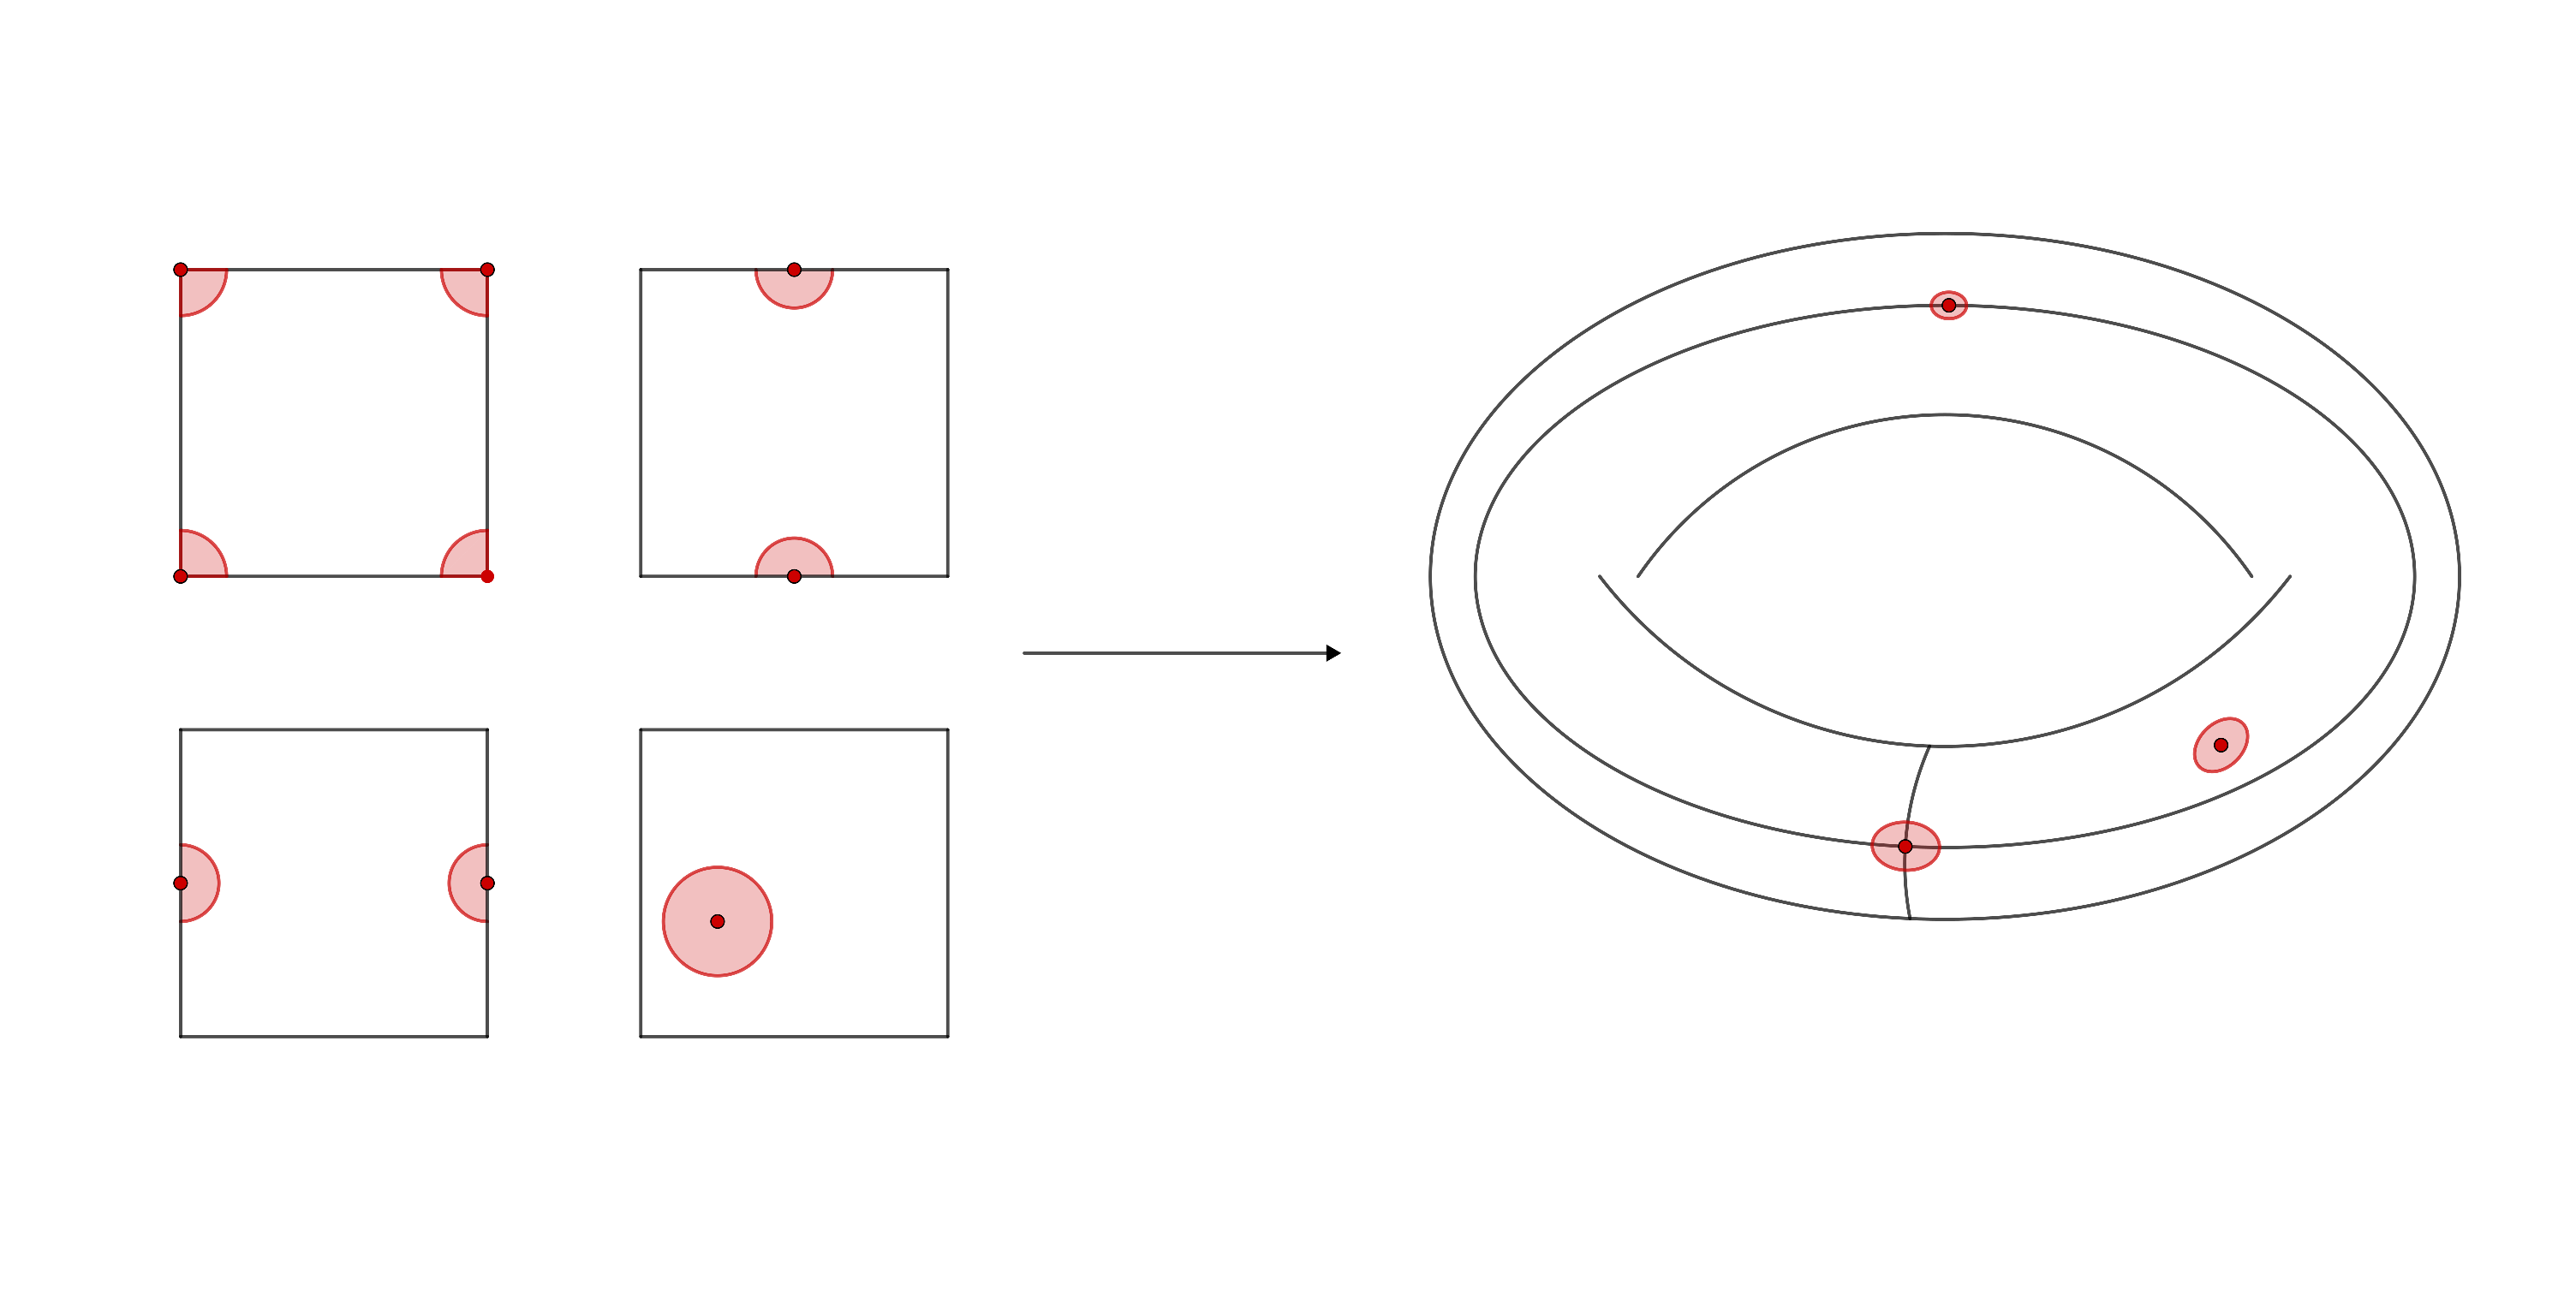
\includegraphics[scale = 0.2]{Figures/Chapter2/squareTorus.eps}
    \caption{Transforming the unit disk into the unit sphere}
    \label{fig_2.4}
\end{figure}

\begin{theorem}\label{2.4.3}
    Let $p:X \rightarrow Y$ be a quotient map and let  $A$ be a subspace of  $X$ saturated with
    respect to  $p$. Let  $q:A \rightarrow p(A)$, then:
        \begin{enumerate}[label=(\arabic*)]
            \item If $A$ is either open or closed, then  $q$ is a quotient map.

            \item If $p$ is either open or closed, then  $q$ is a quotient map.
        \end{enumerate}
\end{theorem}
\begin{proof}
    We first have that $q^{-1}(V)=p^{-1}(V)$ since $V \subseteq A$ and  $A$ is saturated, well
    $p^{-1}(V) \subseteq A$. We also have that $p(U \cap A)=\(U) \cap p(A)$. Now suppose that
    $y=p(u)=p(a)$ for $u \in U$ and  $a \in A$. Since  $A$ is saturated, it contains
    $p^{-1}(p(a))=p^{-1}(p(u))$, hence $y=p(u)$ with $u \in U \cap A$, so  $P(U) \cap p(A) \subseteq
    P(U \cap A)$.

    Now suppose that $A$, or that  $p$ is open. Given  $V \subseteq p(A)$, suppose $q^{-1}(V)
    \subseteq A$ is open. If $A$ is open in $X$, then $q^{-1}(V)$ is also open in $X$, and since
    $q^{-1}(V)=p^{-1}(V)$, then $V$ is open in  $Y$, and since  $p$ is a quotient map, then  $V$ is
    open in  $p(A)$. Now if  $p$ is open, since  $q^{-1}(V)=p^{-1}(V)$ and $q^{-1}(V)$ is open in
    $A$, then  $p^[-1](V)=U \cap A$, thus $V=p(p^{-1}(V))=p(U \cap A)=p(U) \cap p(A)$. Now $p(U)$ is
    open in $Y$, so  $V$ is open in  $p(A)$. In either case e have that $q$ is a quotient map.
\end{proof}

\begin{lemma}\label{2.2.3}
    The composition of two quotient maps is a quotient map,
\end{lemma}
\begin{proof}
    Let $p:X \rightarrow Y$ and  $q:Y \rightarrow Z$ be quotient maps and consider  $q \circ p:X
    \rightarrow Z$. Let $V \subseteq Z$ be open, then  $q^{-1}(V)=U$ is open in $Y$ which implies
    that  $p^{-1}(U)$ is open in $X$. Hence  $p^{-1}(q^{-1}(V))$ is open in $X$.
\end{proof}

\begin{theorem}\label{2.4.5}
    Let $p:X \rightarrow Y$ be a quotient map and let  $Z$ be a topological space with  $g:X
    \rightarrow Z$ a map constant on all  $p^{-1}(\{y\})$ for each $y \in Y$. Then  $g$ induces a
    map $f:Y \rightarrow Z$ such that  $f \circ p=g$, where  $f$ is continuous if and only if  $g$
    is continuous, and where  $f$ is a quotient map if and only if  $g$ is a quotient map.
\end{theorem}

\[\begin{tikzcd}
	X \\
	\\
	Y && Z
	\arrow["g", from=1-1, to=3-3]
	\arrow["f"', dotted, from=3-1, to=3-3]
	\arrow["p"', from=1-1, to=3-1]
\end{tikzcd}\]

\begin{proof}
    For each $y \in Y$, since  $g$ is constant on all  $p^{-1(\{y\})}$, $g(p^{-1(\{y\})})$ is a one
    point set in $Z$; let it be $f(y)$. Then we have a map $f:Y \rightarrow Z$ such that
    $f(p(x))=g(x)$ for each $x$. Now if  $f$ is continuous, then so is  $g$; likewise if  $f$ is a
    quotient map.

    Conversely, suppose that  $g$ is continuous, given  $V \subseteq Z$ open,  $g^{-1}(V)$ is open
    in $X$. Now  $g^{-1}(V)=p^{-1}(f^{-1}(V))$, and since $p$ is a quotient map,  $f^{-1}(V)$ is
    open in $Y$, hence  $f$ is continuous. Now suppose that  $g$ is a quotient map, for  $V
    \subseteq Z$, if  $f^{-1}(V)$ is open in $Y$, then  $p^{-1}(f^{-1}(V))$ is open in $X$ by
    continuity of  $p$, thus  $g^{-1}(V)$ is open in $X$, then  $V$ is open in  $Z$; this makes  $f$
    a quotient map.
\end{proof}
\begin{corollary}
    Let $g:X \rightarrow Z$ be continuous and let $X/\sim=\{g^{-1}(\{z\}):z \in Z\}$ ` be the
    following quotient space for $X$. Then
        \begin{enumerate}[label=(\arabic*)]
            \item The map $g$ induces a continuous  $1-1$ map  $f:X/\sim \rightarrow Z$ of  $X/\sim$
                onto  $Z$ which is a homeomorphism if and only if $g$ is a quotient map.

                \[\begin{tikzcd}
	                X \\
	                \\
	                {X/\sim} && Z
	                \arrow["p"', from=1-1, to=3-1]
	                \arrow["f"', from=3-1, to=3-3]
	                \arrow["g", from=1-1, to=3-3]
                    \end{tikzcd}\]

            \item If $Z$ is Hausdorff, then so is  $X/\sim$.
        \end{enumerate}
\end{corollary}
\begin{proof}
    By the theorem \ref{2.4.5}, $g$ induces a continuous map  $f:X/\sim \rightarrow Z$ which is
    $1-1$ and  (clearly) onto. Suppose that $f$ is a homeomorphism. Then both  $f$ and  $p:X
    \rightarrow X/\sim$ are quotient maps, which makes  $g$ a quotient map. On the other hand, if
    $g$ is a quotient map, then so is  $f$, which makes  $f$  $1-1$ continuous, and hence a
    homeomorphism.

    Now supose that  $Z$ is Hausdorff, given points of  $X/\sim$, their images under  $f$ are
    distinct, and hence they posses disjoint neighborhoods  $U$ and  $V$. Then  $f^{-1}(U) \cap
    f^{-1}(V)=\emptyset$, which makes $X/\sim$ Hausdorff.
\end{proof}

We conclude with some examples.

\begin{example}
    \begin{enumerate}[label=(\arabic*)]
        \item Let $X=\{[0,1] \times n:n \in Z^+\}$ be the subspace of $\R^2$ and let  $Z=\{x \times
            \frac{x}{n}: x \in [0,1] \text{ } n \in \Z^+\}$ be another subspace of $\R^2$. We have
            that  $X$ is the union of countably many disjoint line segments in  $\R^2$ and  $Z$ is
            the union of countably many line segments in  $\R^2$ having a common endpoint.

            Now define $g:X \rightarrow Z$ by  $g:x \times n \rightarrow x \times \frac{x}{n}$. We
            have that $g$ is continous onto. Now consider the quotient space  $X/g$ whose elements
            are  $g^{-1}(\{z\})$ to be the space obtained from $X$ by identifying the equivalence
            classes of $\{0\} \times \Z^+$ to be points. Now we have that $g$ induces a  $1-1$
            continuous map  $f:X/g \rightarrow Z$ of  $X/g$ onto  $Z$; but  $f$ is not a
            homeomorphism. It is sufficient to show that  $g$ is not a quotient mapl consider the
            sequence  $\{\frac{1}{n} \times n\}$ of points of $X$. This sequence is closed in  $X$
            since it has no limit points, it is also saturated with respect to  $g$. However  $g(A)$
            is not closed in $Z$ for it consists of the sequence of points  $\{\frac{1}{n} \times
            \frac{1}{n^2}\}$ whose limit point is the origin (see \ref{fig_2.6}).

            \begin{figure}[h]
                \centering
                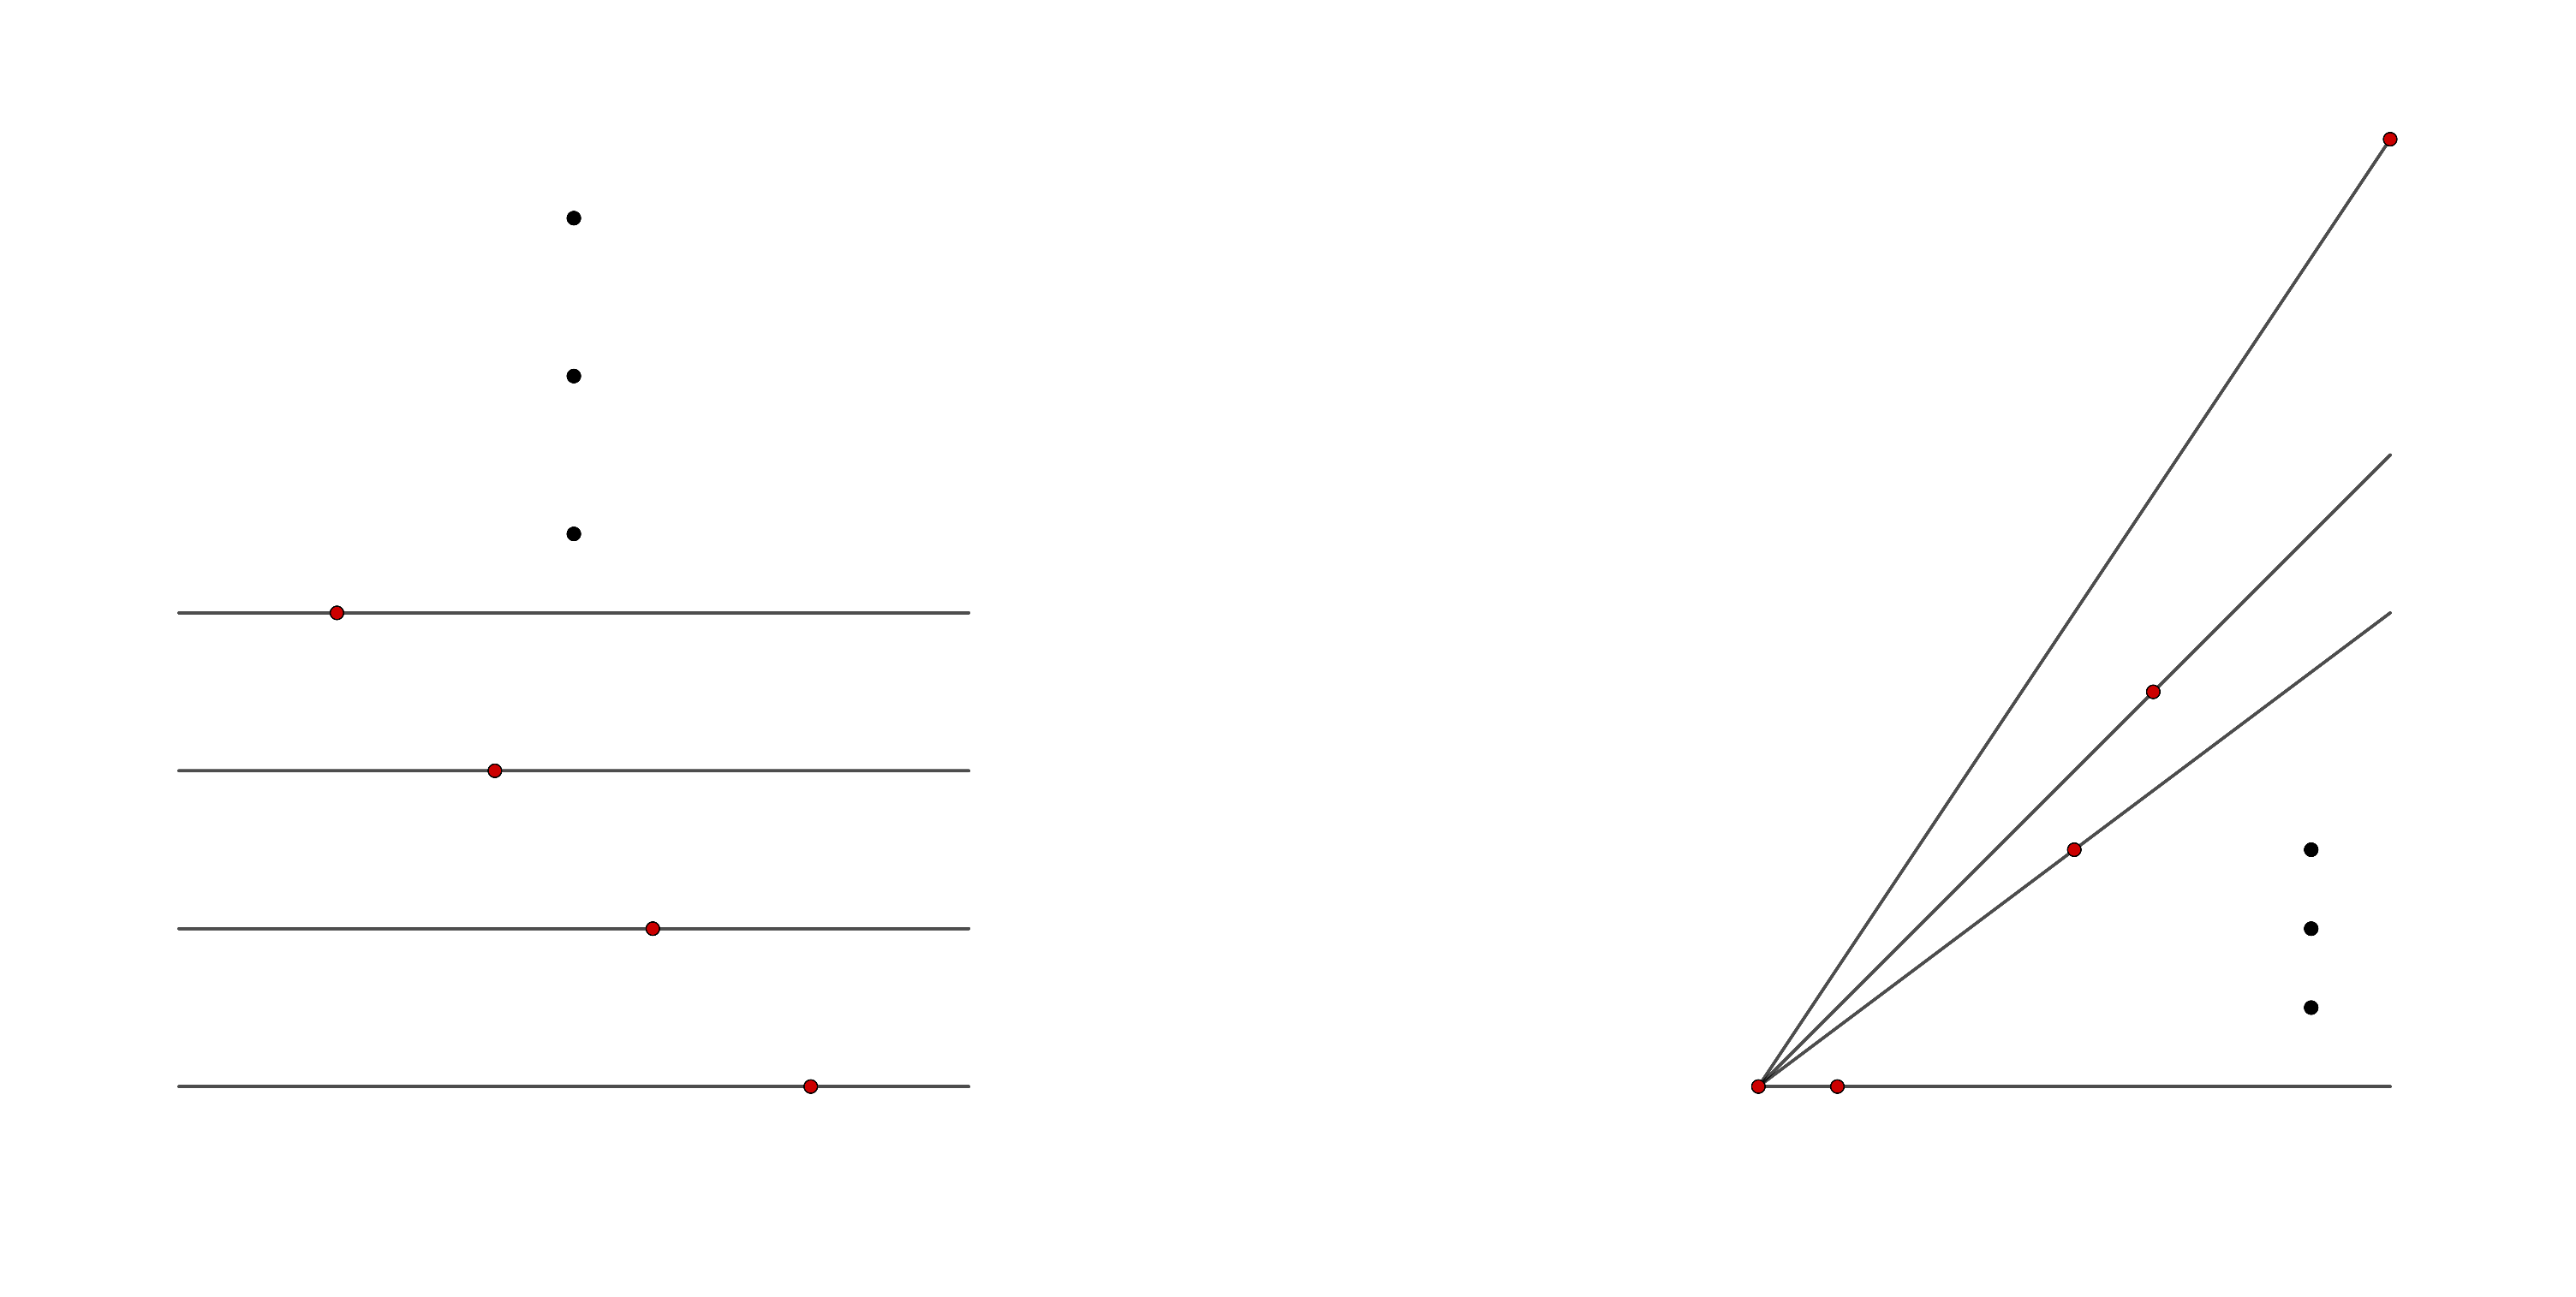
\includegraphics[scale = 0.2]{Figures/Chapter2/nonHomeomorphicPoints.eps}
                \caption{}
                \label{fig_2.6}
            \end{figure}

        \item Not it is not in general true that the product of two quotient maps is itself a
            quotient map. Consider $\R$ and let  $\R/\sim$ be the quotient space obtained from  $\R$
            by taking $\Z^+ \sim b$ for some point  $b$. Now let  $p:\R \rightarrow \R/\sim$ be the
            quotient map and consider  $\Q$ as a subspace of  $\R$. Let  $i:\Q \rightarrow \Q$ be
            the identity map, then  $p \times i:\R \times \Q \rightarrow \R/\sim \times \Q$ is not a
            quotient map. For each  $n$, take the sequence  $\{\frac{\sqrt{2}}{n}\}$ and consider
            the straight lines of slope $\pm1$ in $\R^2$ through the point  $n \times
            \frac{\sqrt{2}}{n}$. Let $U_n$ be the set of all  $\R \times \Q$ points lying above or
            beneth both these line, and between the lines  $x=n \pm \frac{1}{4}$. We have that $U_n$
            is open in  $\R \times Q$ as it contains the set  $\{n\} \times \Q$.

            Now let $U=\bigcup{U_n}$, then $U$ is open in  $\R \times \Q$, and it is saturated with
            respect to  $p \times i$, as  $\Z^+ \times q \in \R \times \Q$ for all  $q \in \Q$, so
            assume that  $U'=p \times i(U)$ is open in $\R/\sim \times \Q$. Now since  $\Z^+ \times
            0 \subseteq U$, the point  $b \times 0 \in U'$, so  $U'$ contains an open set of the
            form  $W \times I_{\delta}$ where $W$ is a neighborhood of  $b$ in  $\R/\sim$, and
            $I_{\delta}=\{y \in \Q:|y|<\delta\}$. Then $p^{-1}(W) \times I_{\delta} \subseteq U$.
            Choosing $n$ large enough so that  $ \frac{\sqrt{2}}{n}<\delta$, since $p^{-1}(W)$ is
            open in $\R$ and contains  $\Z^+$, choose  $0<\epsilon<\frac{1}{4}$ so that
            $(n-\epsilon,n+\epsilon) \subseteq p^{-1}(W)$. Then $U$ contains the subset
            $(n-\epsilon,n+\epsilon) \times I_{\delta} \subseteq \R \times \Q$, however there are
            points that need not lie in $U$, which contradicts that  $U'$ is open in $\R/\sim$ So
            $p \times i$ cannot be a quotient map.
    \end{enumerate}
\end{example} 
